


\chapter{多元微分学}

\section{多变量导数与微分}

\subsection{全微分与偏导数}


\begin{definition}[偏导数]
  $f$在$\mathbf{x}_0 \in D$的偏导数定义为
  $\frac{\partial f}{\partial x_i} := \lim \limits_{t \rightarrow 0} \frac{f(\mathbf{x}_0 + t \mathbf{e}_i) - f(\mathbf{x}_0)}{t}$
\end{definition}

\begin{note}
  计算偏导$f_x(x_0,y_0)$时,预先将$y = y_0$代入,
  得到$f(x,y_0)$,再对$x$求导更加方便。
\end{note}

\begin{definition}[可微]
  若$z = f(x,y)$在$P_0(x_0,y_0)$邻域$U(P_0)$中有定义,
  且对于$U(P_0)$中任意点$(x,y)$,$\exists A,B$使得
  \begin{equation*}
    f(x,y) - f(x_0,y_0) = A(x - x_0) + B(y - y_0) + o(\sqrt{(x - x_0)^2 + (y - y_0)^2})
  \end{equation*}
  则称$f(x,y)$在$P_0$可微。
  可知这里$A = \frac{\partial f}{\partial x}, B = \frac{\partial f}{\partial y}$,
  因此记$\mathrm{d} f(x_0,y_0) = \frac{\partial f}{\partial x}(x_0,y_0)\mathrm{d} x + \frac{\partial f}{\partial y}(x_0,y_0) \mathrm{d} y$
\end{definition}

\begin{note}
  可微定义中的范数可以更改,例如$\Delta z = A \Delta x + B \Delta y + \alpha \Delta x + \beta \Delta y$,
  在$(\Delta x, \Delta y)\rightarrow (0,0)$时$\alpha,\beta \rightarrow 0$,
  该条件也等价于可微。
\end{note}

\begin{corollary}[偏导与可微]
  若$f$在$(x_0,y_0)$可微,
  则$f_x(x_0,y_0), f_y(x_0,y_0)$一定存在
\end{corollary}

\begin{note}
  判断是否可微分两步:
  \begin{enumerate}
  \item 看看$f_x,f_y$是否都存在,不存在则不可微
  \item 计算$\frac{f(x+\Delta x, y + \Delta y) - f(x,y) - f_x\Delta x - f_y\Delta y}{\sqrt{(\Delta x)^2 + (\Delta y)^2}}$是否极限为$0$,是则可微
  \end{enumerate}
\end{note}

~

\begin{exercise}[计算全微分]
  (1)求$u = xe^{yz} + e^{-z} + y$在原点处的全微分
\end{exercise}

\begin{solution}
  (1)原点处$u_x = 1, u_y = 1, u_z = -1$,
  因此原点处$\mathrm{d} u = \mathrm{d} x + \mathrm{d} y - \mathrm{d} z$
\end{solution}

~


\begin{exercise}[判断可微性]
  判断$f(x,y) =
  \begin{cases}
    \frac{xy}{\sqrt{x^2 + y^2}}, & (x,y) \neq (0,0)\\
    0, & (x,y) = (0,0)
  \end{cases}
  $在原点的可微性
\end{exercise}

\begin{solution}
  首先计算偏导,计算$x$偏导时将$y$固定为$0$(而不是固定为一个很小的值!)
  \begin{equation*}
    f_x(0,0) = \frac{f(\Delta x, 0) - f(0,0)}{\Delta x }= 0
  \end{equation*}
  同理可知$f_y(0,0) = 0$,
  再考虑极限
  \begin{equation*}
    \lim \limits _{\rho \rightarrow 0}\frac{f(\Delta x, \Delta y) - f(0,0)-0\Delta x-0 \Delta y}{\sqrt{\Delta x^2 + \Delta y^2}} = \lim \limits _{\rho \rightarrow 0}\frac{\Delta x \Delta y}{\Delta x^2 + \Delta y^2}
  \end{equation*}
  极限不存在,因此不可微。
\end{solution}

\subsection{可微性的证明}

\begin{exercise}[判断可微性]
  (1)讨论$f(x,y) =
  \begin{cases}
    y \ln (x^2 + y^2), & (x,y) \neq (0,0)\\
    0, & (x,y) = (0,0)
  \end{cases}
  $在原点的可微性

  (2)$\alpha > 0$,讨论$f(x,y) = |xy|^{\alpha}$在原点的可微性

  (3)$\alpha > 0$,讨论$f(x,y) =
  \begin{cases}
    \frac{|x|^{\alpha}y}{x^2 + y^2}, & (x,y) \neq (0,0)\\
    0, &(x,y) = (0,0)
  \end{cases}
  $在原点处的可微性
\end{exercise}

\begin{solution}
  (1)先看看偏导数,$f_x(0,0) = \lim \limits _{x \rightarrow 0}\frac{f(x,0) - f(0,0)}{x} = \frac{0}{x} = 0$,
  $f_y(0,0) = \lim \limits _{y \rightarrow 0}\frac{y \ln(y^2) - 0}{y} = -\infty$,因此不可微

  (2)先看看偏导数$f_x(0,0) = \lim \limits _{x \rightarrow 0}\frac{0}{x} = 0$,
  $f_y(0,0) = \lim \limits _{y \rightarrow 0}\frac{0}{y} = 0$,
  考虑:
  \begin{equation*}
    \frac{f(x,y) - f(0,0) - f_x(0,0) x - f_y(0,0)y}{\sqrt{x^2 + y^2}} = \frac{|xy|^{\alpha}}{\sqrt{x^2 + y^2}}
  \end{equation*}
  考察上述分式是否趋于$0$,
  用极坐标变换即可得出
  若$\alpha > \frac{1}{2}$,则可微,
  若$0 < \alpha \leq \frac{1}{2}$,则不可微

  (3)$f_x(0,0) = f_y(0,0) = 0$,
  而$\frac{f(x,y)}{\sqrt{x^2 + y^2}} =  \frac{|x|^{\alpha} y}{(x^2 + y^2)^{\frac{3}{2}}}$,
  使用极坐标变换得到
  $r^{\alpha - 2} |\cos \theta|^{\alpha} \sin \theta$。
  因此$\alpha > 2$时可微,$0 < \alpha \leq 2$时不可微(例如取$\theta = \frac{\pi}{4}$)。
\end{solution}


\subsection{梯度与方向导数}

\begin{definition}[梯度]
  对于$f:\mathbb{R}^n \rightarrow \mathbb{R}$,
  定义梯度$\nabla f := [\frac{\partial f}{\partial x_1}, \frac{\partial f}{\partial x_2},\cdots,\frac{\partial f}{\partial x_n}]^T$
\end{definition}

\begin{definition}[方向导数]
  开集$D \subset \mathbb{R}^n, f:D \rightarrow \mathbb{R}$,
  $\mathbf{u} \in \mathbb{R}^n$为单位向量,$\mathbf{x}_0 \in D$,
  定义$\frac{\partial f}{\partial \mathbf{u}} := \lim \limits _{t \rightarrow 0} \frac{f(\mathbf{x}_0 + t\mathbf{u}) - f(\mathbf{x}_0)}{t}$
\end{definition}

\begin{note}
  要计算方向导数,则可取方向为$(\cos \alpha, \cos \beta)$,且$\cos^2\alpha + \cos^2\beta = 1$。
  原因在于$\frac{(x - x_0, y - y_0)}{|(x-x_0,y-y_0)|} = \frac{1}{r}(x - x_0,y - y_0) = (\cos \alpha, \cos \beta)$
\end{note}

~

\begin{exercise}[常用反例]
  (1)证明$f(x,y) = \sqrt[3]{x^2 + y^2}$在原点连续,但不存在任意方向导数和偏导数
\end{exercise}

\begin{proof}
  (1)考虑方向$l = (\cos \alpha, \cos \beta)$,
  则$f_l(0,0) = \lim \limits _{r \rightarrow 0^+}\frac{f(r \cos \alpha, r\cos \beta) - f(0,0)}{r} = \lim \limits _{r \rightarrow 0^+} \frac{1}{r^{1/3}} = \infty$
\end{proof}

~

\begin{theorem}[可微函数方向导数的梯度表达]
  若$f(x,y)$在$P_0(x_0,y_0)$可微,则$f(x,y)$在$P_0$沿任一方向$l$的方向导数存在,且
  \begin{equation*}
    f_l(P_0) = f_x(P_0)\cos \alpha + f_y(P_0)\cos \beta = \nabla f \cdot \mathbf{n}
  \end{equation*}
  这里$\mathbf{n} = (\cos \alpha, \cos \beta)$是$l$方向的单位向量
\end{theorem}

\begin{proof}
  考虑方向导数$f_l(P_0) = \lim \limits _{r \rightarrow 0^+} \frac{f(x_0 + r\cos \alpha , y_0 + r \cos \beta) - f(x_0,y_0)}{r}$,可化简为:
  \begin{equation*}
     \lim \limits _{r \rightarrow 0^+} \frac{f_x(x_0,y_0) r \cos \alpha + f_y(x_0,y_0)r \cos \beta + o(r)}{r} = f_x(x_0,y_0) \cos \alpha + f_y(x_0,y_0)\cos \beta
  \end{equation*}
\end{proof}

\begin{note}
  设$\theta$是$\nabla f$与$l$的夹角,
  则$f_l(\mathbf{x}_0) = |\nabla f| |\mathbf{n}| \cos \theta = |\nabla f| \cos \theta$。
  可知梯度方向是增长最快的方向。
\end{note}

~

\begin{exercise}[梯度与方向导数计算]
  (1)计算$u = xyz$在$A(5,1,2)$朝向$B(9,4,14)$的方向导数

  (2)$u(x,y,z) = xy^2z^3$,求$u(x,y,z)$在$(1,1,1)$处函数值增长最快的方向
\end{exercise}

\begin{solution}
  (1)可微函数具体计算方向导数时一般用$\nabla f \cdot \mathbf{n}$计算。
  $\overrightarrow{AB} = (4,3,12)$,
  因此$\mathbf{n} = \frac{1}{13}(4,3,12)$,
  $A$处梯度为$(2,10,5)$,
  因此$\nabla f \cdot \mathbf{n} = \frac{1}{13}(8 + 30 + 60) = \frac{98}{13}$

  (2)即梯度方向,
  $u_x = y^2z^3, u_y = 2xyz^3, u_z = 3xy^2z^2$,
  因此梯度为$(1,2,3)$
\end{solution}

~

\begin{exercise}[方向导数的应用]
  已知$f(x,y)$可微,若$l_1,l_2$是$\mathbb{R}^2$上一组线性无关的向量,
  若$f_{l_1}(x,y) = f_{l_2}(x,y) \equiv 0$,证明$f(x,y)$为常值函数。
\end{exercise}

\begin{proof}
  不妨设$n_{l_1} = (\cos \alpha, \sin \alpha), n_{l_2} = (\cos \beta, \sin \beta)$,
  此时根据条件
  \begin{equation*}
    \begin{cases}
      f_{l_1} = f_x \cos \alpha + f_y \sin \alpha \equiv 0\\
      f_{l_2} = f_x \cos \beta + f_y \sin \beta \equiv 0
    \end{cases}
  \end{equation*}
  根据线性无关条件可解出$f_x \equiv f_y \equiv 0$,
  因此为常值函数。
\end{proof}


\subsection{可微、偏导、方向导数、连续关系总结}

\begin{theorem}[可微的性质]
  若$f$在$\mathbf{x}_0$可微,则
  \begin{itemize}
  \item $f$在$\mathbf{x}_0$处连续
  \item $f$在$\mathbf{x}_0$处存在偏导数和任意方向导数
  \end{itemize}
\end{theorem}

\begin{proof}
  (1)根据定义显然$||\mathbf{h}|| \rightarrow 0$时,$f(\mathbf{x} + \mathbf{h}) - f(\mathbf{x}) \rightarrow 0$,
  因此连续
\end{proof}

\begin{theorem}[可微充分条件]
  若$f(x,y)$偏导数$f_x,f_y$在$(x_0,y_0)$连续,则$f(x,y)$在$(x_0,y_0)$可微
\end{theorem}

\begin{proof}
  首先写为$\Delta z = [f(x_0+\Delta x, y_0 + \Delta y) - f(x_0 , y_0 + \Delta y)] + [f(x_0,y_0 + \Delta y) - f(x_0,y_0)]$,根据Lagrange中值定理得到
  \begin{equation*}
    \Delta z = f_x(x_0+\theta_1 \Delta x, y_0 + \Delta y)\Delta x + f_y(x_0, y_0 + \theta_2 \Delta y) \Delta y
  \end{equation*}
  根据偏导连续,$\exists \alpha, \beta$在$(\Delta x, \Delta y) \rightarrow (0,0)$时$\alpha, \beta \rightarrow 0$,
  满足
  \begin{equation*}
    \begin{cases}
      f_x(x_0 + \theta_1 \Delta x, y_0 + \Delta y) = f_x(x_0,y_0) + \alpha\\
      f_y(x_0,y_0 + \Delta y) = f_y(x_0,y_0) + \beta
    \end{cases}
  \end{equation*}
  得到$\Delta z = f_x(x_0,y_0) \Delta x + f_y(x_0,y_0)\Delta y + \alpha \Delta x + \beta \Delta y$,即可微。
\end{proof}

\begin{note}
  若$f_x,f_y$连续,则一般称$f(x,y)$连续可微。
\end{note}

\begin{theorem}[偏导与方向导的性质]
  偏导与方向导数相关性质:
  \begin{itemize}
  \item 若$f$偏导数在$(x_0,y_0)$邻域有界,则$f$在$(x_0,y_0)$连续
  \item $f$的偏导数存在或任意方向导数存在并不能推出连续或可微
  \end{itemize}
\end{theorem}

\begin{proof}
  (1)首先$f(x,y) - f(x_0,y_0) = f(x,y) - f(x_0,y) + f(x_0,y) - f(x_0,y_0)$,
  根据Lagrange中值定理得到
  \begin{equation*}
    f(x,y) - f(x_0,y) = f_x(\xi,y)(x-x_0), \quad f(x_0,y) - f(x_0,y_0) = f_y(x_0,\eta)(y-y_0)
  \end{equation*}
  根据偏导有界条件,
  因此$|f(x,y) - f(x_0,y_0)| \rightarrow 0$,因此连续。

  (2)均见下面的重要反例
\end{proof}

~


\begin{exercise}[方向导数、偏导数存在,但不可微,不连续例子]
  证明下面的$f(x,y)$在原点不连续,但是$f_x(0,0) = f_y(0,0) = 0$,
  任何方向$l$满足$f_l(0,0) = 0$,
  \begin{equation*}
    f(x,y) =
    \begin{cases}
      1, & 0 < y < x^2 , -\infty < x < \infty\\
      0, &\text{其他}
    \end{cases}
  \end{equation*}
\end{exercise}

\begin{proof}
  不连续的原因是可以选择$0$趋近,也可以选择$1$趋近。
  但方向导数都为$0$的原因是$y = x^2$在原点处切线是水平的,无论原点处切线取什么,都会经过$0$区域。
\end{proof}


~
\subsection{复合求导:链式法则}

\begin{theorem}[链式法则]
  若$x = \varphi(x,t), y = \psi(s,t)$在$(s,t) \in D$可微,
  $z = f(x,y)$在$(x,y) = (\varphi(s,t), \varphi(s,t))$可微,则复合函数$z = f(\varphi(s,t), \psi(s,t))$在
  $(s,t)$可微,且
  \begin{equation*}
    \begin{cases}
      \frac{\partial z}{\partial s} \bigg|_{(s,t)} = \frac{\partial z }{\partial x} \bigg|_{(x,y)} \frac{\partial x}{\partial s}\bigg|_{(s,t)} + \frac{\partial z}{\partial y}\bigg|_{(x,y)} \frac{\partial y}{\partial s}\bigg|_{(s,t)}\\
      \frac{\partial z}{\partial t} \bigg|_{(s,t)} = \frac{\partial z }{\partial x} \bigg|_{(x,y)} \frac{\partial x}{\partial t}\bigg|_{(s,t)} + \frac{\partial z}{\partial y}\bigg|_{(x,y)} \frac{\partial y}{\partial t}\bigg|_{(s,t)}
    \end{cases}
  \end{equation*}
\end{theorem}

~

\begin{exercise}[链式法则练习]
  (1)设$z = uv + \sin t$,其中$u = e^t, v = \cos t$,计算$\frac{\mathrm{d} z}{\mathrm{d} t}$

  (2)计算$x^x$的导数
\end{exercise}

\begin{solution}
  (1)展开后如下:
  \begin{align*}
    \frac{\mathrm{d} z }{\mathrm{d} t} &= \frac{\partial z}{\partial u} \frac{\mathrm{d} u}{\mathrm{d} t} + \frac{\partial z}{\partial v}\frac{\mathrm{d}v}{\mathrm{d} t} + \frac{\partial z}{\partial t}\\
    &= ve^t + u(-\sin t) + \cos t = e^t(\cos t - \sin t) + \cos t
  \end{align*}

  (2)可以两边取对数隐函数求导。
  或者令$y = u^v$,
  则$\frac{\mathrm{d} y}{\mathrm{d} x} = u^v \ln u + v (u^{v-1}) = x^x(1 + \ln x)$
\end{solution}

~

\begin{exercise}[高阶偏导]
  (1)设$z = f \left( x, \frac{x}{y} \right)$,求$\frac{\partial^2 z}{\partial x^2}, \frac{\partial^2 z}{\partial x \partial y}$。
\end{exercise}

\begin{solution}
  把每个位置当作一层参数即可,注意偏导的参数仍保持一致

  (1)$\frac{\partial z}{\partial x} = f_1(x, \frac{x}{y}) + f_2(x,\frac{x}{y}) \frac{1}{y}$,
  因此
  \begin{equation*}
    \frac{\partial^2 z }{\partial x^2} = f_{11} + f_{12}\frac{1}{y} + \left[ f_{21}+f_{22}\frac{1}{y} \right]\frac{1}{y} = f_{11} + \frac{2}{y}f_{12}+\frac{1}{y^2}f_{22}
  \end{equation*}
\end{solution}



\subsection{混合偏导}

\begin{theorem}[混合偏导定理]
  若$f_{xy}(x,y), f_{yx}(x,y)$均在$x_0,y_0$邻域连续,则
  \begin{equation*}
    f_{xy}(x_0,y_0) = f_{yx}(x_0,y_0)
  \end{equation*}
\end{theorem}

\begin{proof}
  定义$F(\Delta x, \Delta y) = f(x_0 + \Delta x, y_0 + \Delta y) - f(x_0 + \Delta x, y_0) - f(x_0,y_0 + \Delta y) + f(x_0,y_0)$,
  则
  \begin{equation*}
    F(\Delta x, \Delta y) =
    \begin{cases}
      [f_x(x_0 + \theta_1 \Delta x, y_0 + \Delta y) - f_x(x_0 + \theta_1 \Delta x, y_0)]\Delta x\\
      [f_y(x_0 + \Delta x, y_0 + \theta_2 \Delta y) - f_y(x_0,y_0 + \theta_2\Delta y)]\Delta y
    \end{cases}
  \end{equation*}
  再根据Lagrange中值定理:
  \begin{equation*}
    F(\Delta x, \Delta y) =
    \begin{cases}
      f_{xy}(x_0 + \theta_1 \Delta x, y_0 + \theta_3 \Delta y)\Delta x \Delta y\\
      f_{yx}(x_0 + \theta_4\Delta x, y_0 + \theta_2 \Delta y)\Delta x \Delta y
    \end{cases}
  \end{equation*}
  因此$\frac{F(\Delta x, \Delta y)}{\Delta x \Delta y} = f_{xy}(x_0 + \theta_1 \Delta x, y_0 + \theta_3 \Delta y) = f_{yx}(x_0 + \theta_4 \Delta x, y_0 + \theta_2 \Delta y)$,
  令$\Delta x, \Delta y \rightarrow 0$即可得到结果。
\end{proof}

~

\begin{exercise}[混合偏导不相同的例子]
  对于下面的函数,$f_{xy}(0,0) \neq f_{yx}(0,0)$:
  \begin{equation*}
    f(x,y) =
    \begin{cases}
      xy \frac{x^2 - y^2}{x^2 + y^{2}}& (x,y) \neq (0,0)\\
      0, & (x,y) = (0,0)
    \end{cases}
  \end{equation*}
\end{exercise}

\begin{solution}
  直接计算可以得到$f_{xy}(0,0) = -1, f_{yx}(0,0) = 1$
\end{solution}

~

\begin{exercise}[混合偏导相关练习]
  (1)设$f_x,f_y,f_{yx}$在$(x_0,y_0)$邻域存在,$f_{yx}$在$(x_0,y_0)$连续,
  证明$f_{xy}(x_0,y_0)$也存在,且$f_{xy}(x_0,y_0) = f_{yx}(x_0,y_0)$

  (2)设$f_x, f_y$在$(x_0,y_0)$某邻域存在且在$(x_0,y_0)$可微,证明:
  $f_{xy}(x_0,y_0) = f_{yx}(x_0,y_0)$
\end{exercise}





\section{多元中值定理与泰勒展开}

\subsection{多元中值定理}

\begin{definition}[凸区域]
  区域$D \subset \mathbb{R}^2$,
  若$\forall P_1(x_1,y_1), P_2(x_2,y_2) \in D$和$\forall \lambda \in [0,1]$满足
  \begin{equation*}
    (x_1 + \lambda(x_2 - x_1), y_1 + \lambda(y_2 - y_1)) \in D
  \end{equation*}
  即任意两点的连线都含于$D$,则称$D$为凸区域。
\end{definition}

\begin{figure}[htp]
  \centering
  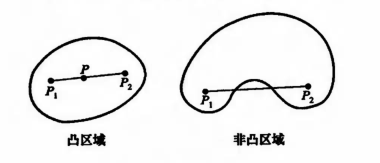
\includegraphics[width=0.5\textwidth]{凸区域.png}
  \caption{凸区域}
\end{figure}

\begin{theorem}[多元中值定理]
  二元函数$f(x,y)$在凸开域$D \subset \mathbb{R}^2$连续,在$D$内点均可微,
  则对$\forall P(a,b), Q(a + h, b + k) \in D$,$\exists \theta \in (0,1)$满足
  \begin{equation*}
    f(a+h,b+k) -f(a,b) = f_x(a + \theta h, b + \theta k)h + f_y(a+\theta h, b + \theta k)k
  \end{equation*}
\end{theorem}

\begin{proof}
  令$\Phi(t) = f(a + th, b + tk)$,
  根据Lagrange中值定理得到$\exists \theta \in (0,1)$使得$\Phi(1) - \Phi(0) = \Phi^{\prime}(\theta)$,而
  \begin{equation*}
    \Phi^{\prime}(\theta) = f_x(a + \theta h, b + \theta k)h + f_y(a + \theta h, b + \theta k)k
  \end{equation*}
  由于$D$是凸区域,因此$(a + \theta h, b + \theta k ) \in D$,从而结论成立。
\end{proof}

\subsection{多元Taylor展开}

\begin{theorem}[多元Taylor展开]
  多元泰勒$f(x + \Delta x, y + \Delta y)$展开的公式如下:
  \begin{equation*}
    f(x,y) + \sum\limits_{l = 1}^n \frac{1}{l!}\left( {l \choose 0} \frac{\partial ^l f}{\partial y^l}(x,y) \Delta y^l + {l \choose 1}\frac{\partial^l f}{\partial x \partial y^{l-1}}(x,y)\Delta x \Delta y^{l-1} + \cdots + {l \choose l }\frac{\partial^l f}{\partial  x^l}(x,y) \Delta x^l\right) + R(\Delta x,\Delta y)
  \end{equation*}
\end{theorem}

\begin{proof}
  设$\Phi(t) = f(x_0 + th, y_0 + tk)$,用一元Taylor公式证明。
\end{proof}

\section{隐函数定理}

\subsection{隐函数存在定理与可微定理}

隐函数研究的问题是给定一个二维曲线表达式$F(x,y) = 0$,
希望研究$y = y(x)$的存在性,并计算$y^{\prime}(x)$,
而计算$y^{\prime}(x)$其实不需要得到$y(x)$的具体表达式,
因此隐函数求导大幅度简化了求导过程,因此作为多元微分学的一部分。

\begin{definition}[隐函数]
  $E \subset \mathbb{R}^2$,$F: E \rightarrow \mathbb{R}$,
  对于方程$F(x,y) = 0$,
  若存在集合$I,J \subset \mathbb{R}$使得$\forall x \in I$存在唯一$y \in \mathbb{R}$,
  满足$F(x,y) = 0$,则称$F(x,y) = 0$定义了隐函数。
\end{definition}

\begin{theorem}[隐函数存在唯一性定理]
  若$F(x,y)$满足
  \begin{enumerate}
  \item 
    $F$在$P_0(x_0,y_0)$为内点的某一区域$D$存在$x,y$连续偏导
  \item 
    $F(x_0,y_0) = 0$,且$F_y(x_0,y_0) \neq 0$
  \end{enumerate}
  则:
  \begin{enumerate}
  \item $F(x,y) = 0$唯一定义了$\forall x \in U(x_0, \delta)$上的连续函数$y = f(x)$
  \item $f(x)$在$U(x_0,\delta)$上连续可微,且$f^{\prime}(x) = - \frac{F_x(x,y)}{F_y(x,y)}$(这里$F_x$求导时把$y$当作常数而非函数!)
  \item 特别地,对于$F(x_1,\cdots,x_n,y) = 0$,$y = f(x_1,\cdots,x_n)$,得到$f_{x_i}(x_1,\cdots,x_n) = - \frac{F_{x_i}}{F_y}$
  \end{enumerate}
\end{theorem}

\begin{proof}
  (2)$F(x,y) = 0$两侧对$x$求导得到$F_x(x,y) + F_y(x,y)y^{\prime} = 0$,
  因此$y^{\prime} = - \frac{F_x(x,y)}{F_y(x,y)}$
\end{proof}

\begin{note}
  如果只希望得到$f(x)$连续,则条件可减弱为$F(x,y)$在$P_0(x_0,y_0)$某邻域连续,
  $F(x_0,y_0) = 0$,固定$x$时$F(x,y)$关于$y$严格单调。
\end{note}

\begin{note}
  若要求高阶导,则可以对$y^{\prime} = - \frac{F_x}{F_y}$两边求导,再将$y^{\prime}(x)$表达式带进去,
  或者实际计算时可以$F(x,y) = 0$直接两边求两次导。
\end{note}

~

\begin{exercise}[隐函数求导]
  (1)$y = y(x)$由$\ln \sqrt{x^2 + y^2} = \arctan \frac{y}{x}$确定,求$\frac{\mathrm{d} y}{\mathrm{d} x}$

  (2)$z = z(x,y)$由$F(x-y,y-z) = 0$所确定的隐函数,求$z_x,z_y,z_{xy}$

  (3)$F(x,y,z) = 0$可以确定$z = z(x,y), y = y(z,x), x = x(y,z)$,证明:$\frac{\partial x}{\partial y} \cdot \frac{\partial y}{\partial z} \cdot \frac{\partial z}{\partial x} = -1$
\end{exercise}

\begin{solution}
  (1)可以用隐函数求导公式,此时$F$对$x,y$求导时,将它们视为彼此无关的:
  \begin{equation*}
    \begin{cases}
      F_x = \frac{x}{x^2 + y^2} - \frac{-\frac{y}{x^2}}{1 + \left( \frac{y}{x} \right)^2} = \frac{x+y}{x^2 + y^2}\\
      F_y = \frac{y-x}{x^2 + y^2}
    \end{cases} \Rightarrow \frac{\mathrm{d} y}{\mathrm{d} x} = \frac{x+y}{x-y}
  \end{equation*}
  或者直接两侧求导,此时视$y = y(x)$与$x$有关:
  \begin{equation*}
    \frac{x}{x^2 + y^2} + \frac{y}{x^2 + y^2}\cdot y^{\prime} + \frac{y}{x^2 + y^2} + \frac{x}{x^2 + y^2}\cdot y^{\prime} = 0
  \end{equation*}

  (2)比较难用隐函数求导公式,只能两边求导。
  视$z = z(x,y)$,$x,y$彼此无关,则
  两侧分别对$x,y$求导得到:
  \begin{equation*}
    \begin{cases}
      F_1 + F_2(- z_x) = 0 \Rightarrow z_x = \frac{F_1}{F_2}\\
      -F_1 + F_2(1 - z_y) = 0 \Rightarrow z_y =1 - \frac{F_1}{F_2}
    \end{cases}
  \end{equation*}
  要求$z_{xy}$,可以对$F_1(x-y,y-z)- z_x F_2(x-y,y-z) = 0$两侧对$y$求导,
  得到
  \begin{equation*}
    \left( - F_{11} + F_{12}(1 - z_y) \right) - \left( F_{21}(-1) + F_{22}(1 - z_y) \right)z_x - F_2 z_{xy} = 0 \Rightarrow z_{xy} = \frac{2F_1F_2F_{12} - F_{11}F_2^2 - F_{22}F_1^2}{F_2^3}
  \end{equation*}

  (3)注意这里的符号含义,不能简简单单乘起来变成$1$。
  例如$\frac{\partial x}{\partial y}$的含义为$\frac{\partial x(y,z)}{y}$,
  因此根据隐函数定理即
  \begin{equation*}
    -\frac{F_y}{F_x} \cdot - \frac{F_z}{F_y} \cdot - \frac{F_x}{F_z} = -1
  \end{equation*}
\end{solution}



\subsection{隐函数组存在定理与微分定理}

\begin{theorem}[隐函数组定理]
  若$F(x,y,u,v), G(x,y,u,v)$满足:
  \begin{itemize}
  \item 在$P_0(x_0,y_0,u_0,v_0)$邻域中对所有变量有连续偏导
  \item $F(P_0) = G(P_0) = 0$,$J = \frac{\partial(F,G)}{\partial(u,v)}\bigg|_{P_0} \neq 0$
  \end{itemize}
  则方程组
  \begin{equation*}
    \begin{cases}
      F(x,y,u,v) = 0\\
      G(x,y,u,v) = 0
    \end{cases}
  \end{equation*}
  在$P_0$邻域中唯一确定了两个二元连续隐函数$u = f(x,y), v = g(x,y)$,设$J = \frac{\partial(F,G)}{\partial(u,v)}$,则
  \begin{equation*}
    u_x = - \frac{1}{J} \frac{\partial(F,G)}{\partial(x,v)}, u_y = - \frac{1}{J} \frac{\partial(F,G)}{\partial(y,v)}, v_x = - \frac{1}{J} \frac{\partial(F,G)}{\partial(u,x)}, v_y = - \frac{1}{J} \frac{\partial(F,G)}{\partial(u,y)}
  \end{equation*}
  记忆口诀为求什么就换什么,例如求$u_x$就把$\frac{\partial(F,G)}{\partial(u,v)}$中的$u$换成$x$,
  得到$\frac{\partial(F,G)}{\partial(x,v)}$
\end{theorem}

\begin{proof}
  求导结论使用了Cramer法则
\end{proof}

\begin{note}
  一般而言有几个方程就有几个因变量,其余的为自变量。
\end{note}

\begin{exercise}[容易分不清的题]
  (1)错过:已知$x = \varphi(t), y = \phi(x)$,
  $\varphi^{\prime}(t) = e^t + 1, \frac{\mathrm{d} ^3y}{\mathrm{d}x^3} = e^t + 2t$,
  求$\frac{\mathrm{d} ^4y}{\mathrm{d} x^4}$
\end{exercise}

\begin{solution}
  (1)直接求:
  \begin{equation*}
    \frac{\mathrm{d}^4y}{\mathrm{d} x^4} = \frac{\left( \frac{\mathrm{d}^3y}{\mathrm{d}x^3} \right)/ \mathrm{d} t}{\mathrm{d} x /\mathrm{d} t} = \frac{e^t + 2}{e^t + 1}
  \end{equation*}
\end{solution}

~

\begin{exercise}[隐函数组求导]
  (1)证明
  \begin{equation*}
    \begin{cases}
      x^2 + y^2 + u^2 - v^2 = 2\\
      x+y+u+v = 0
    \end{cases}
  \end{equation*}
  在$P_0(1,1,-1,-1)$的某邻域中能确定隐函数组$u = u(x,y), v = v(x,y)$,并求$\frac{\partial u}{\partial x}, \frac{\partial v}{\partial y}$

  (2)设$u = u(x,y), v = v(x,y)$由方程组
  \begin{equation*}
    \begin{cases}
      u = f(ux,v+y)\\
      v = g(u-x,v^2y)
    \end{cases}
  \end{equation*}
  给出的隐函数,求$u_x, v_x$

  (3)已知如下方程组,求$z_x$:
  \begin{equation*}
    \begin{cases}
      x = u+v\\
      y = u^2 + v^2\\
      z = u^3 + v^3
    \end{cases}
  \end{equation*}

  (4)令$u = f(x-ut, y-ut, z - ut), g(x,y,z) = 0$,求$u_x,u_y$
\end{exercise}

\begin{solution}
  (1)$F = x^2 + y^2 + u^2 - v^2 - 2, G = x+y+u+v$,
  则显然$F,G$对每个分量都有连续偏导数,$F(P_0) = G(P_0) = 0$,
  方便起见,直接求出所有偏导:
  \begin{equation*}
    \left[
      \begin{array}{cccc}
        F_x&F_y&F_u&F_v \\
           G_x&G_y&G_u&G_v
      \end{array}
    \right] = \left[
      \begin{array}{cccc}
        2x&2y&2u&-2v \\
          1&1&1&1
      \end{array}
    \right] \Rightarrow \frac{\partial(F,G)}{\partial(u,v)} = \left|
      \begin{array}{cc}
        2u&-2v \\
          1&1
      \end{array}
    \right| = 2v + 2u
  \end{equation*}
  因此$J(P_0) \neq 0$,隐函数组存在,
  根据隐函数组求导:
  \begin{equation*}
    \frac{\partial u}{\partial x} = - \frac{1}{J} \frac{\partial(F,G)}{\partial(x,v)} = - \frac{1}{2u+2v} \cdot(2x + 2v) = - \frac{x+v}{u+v},
    \frac{\partial v}{\partial y} = - \frac{y - u}{u + v}
  \end{equation*}

  (2)直接两侧求导,得到
  \begin{equation*}
    \begin{cases}
      u_x = f_1\cdot(u_xx + u) + f_2v_x \Rightarrow (1 - xf_1)u_x - f_2 v_x = uf_1\\
      v_x = g_1\cdot (u_x - 1) + g_2 2vv_xy \Rightarrow g_1u_x + (2vyg_2 - 1)v_x = g_1
    \end{cases}
  \end{equation*}
  解线性方程组得到
  \begin{equation*}
    u_x = \frac{(2vyg_2 - 1)uf_1 + f_2g_1}{(1 - xf_1)(2vyg_2 - 1)+f_2g_1}, v_x = \frac{(1 - xf_1)g_1 - uf_1g_1}{(1 - xf_1)(2vyg_2 - 1) + f_2g_1}
  \end{equation*}

  (3)令$x,y$为自变量,$u,v,z$为因变量,则
  \begin{equation*}
    z_x = -\frac{ \frac{\partial(F,G,H)}{\partial(x,u,v)}}{\frac{\partial(F,G,H)}{\partial(z,u,v)}}
  \end{equation*}
\end{solution}

\section{多元无条件极值问题}


\begin{definition}[极值与极值点]
  开集$D\subset \mathbb{R}^n$,
  函数$f: D \rightarrow \mathbb{R}$,
  $x_0 \in D$,
  若存在球$B_r(x_0) \subset D$使得$\forall x \in B_r(x_0)$有$f(x) \geq f(x_0)$,
  则称$x_0$为$f$的一个极小值点。
\end{definition}

\begin{definition}[驻点、稳定点]
  若$P_0(x_0,y_0)$满足$f_x(x_0,y_0) = f_y(x_0,y_0) = 0$,
  则称其为$f(x,y)$的驻点/稳定点。
\end{definition}

\begin{definition}[Hesse矩阵]
  $f:\mathbb{R}^n \rightarrow \mathbb{R}$,
  则其Hesse矩阵为:
  \begin{equation*}
    H = \left[
      \begin{array}{cccc}
        \frac{\partial^2 f}{\partial x_1^2}& \frac{\partial^2 f}{\partial x_1\partial x_2}& \cdots&\frac{\partial^2 f}{\partial x_1\partial x_n}\\
        \frac{\partial^2 f}{\partial x_2 \partial x_1}&\frac{\partial^2 f}{\partial x_2^2}&\cdots & \frac{\partial^2 f}{\partial x_2 \partial x_n}\\
        \vdots&\vdots&\ddots&\vdots\\
        \frac{\partial^2 f}{\partial x_n \partial x_1}& \frac{\partial^2 f}{\partial x_n \partial x_2}&\cdots & \frac{\partial^2 f}{\partial x_n^2}
      \end{array}
    \right]
  \end{equation*}
\end{definition}

\begin{definition}[正定、负定、不定]
  矩阵$A$是对称矩阵,考虑$Q(x) = \mathbf{x}^TA\mathbf{x}$,分为以下三种情况:
  \begin{itemize}
  \item 正(负)定:对$\forall \mathbf{x}, Q(\mathbf{x}) \geq(\leq) 0$
  \item 不定:$\exists \mathbf{p},\mathbf{q} \in \mathbb{R}^n$,$Q(\mathbf{p}) \leq 0 \leq Q(\mathbf{p})$
  \end{itemize}
\end{definition}

\begin{theorem}[正定的判别法]
  $A$为对称矩阵,则$A$严格正定当且仅当其各阶顺序主子式均大于$0$
\end{theorem}

\subsection{无条件极值}

\begin{theorem}[极值点必要条件]
  若$f(x,y)$在$P_0(x_0,y_0)$存在偏导数,
  且在$P_0$取到极值,
  则$f_x(x_0,y_0) = f_y(x_0,y_0) = 0$
\end{theorem}

\begin{proof}
  用反证法即可。
\end{proof}

\begin{theorem}[极值点充分条件]
  $f:\mathbb{R}^2 \rightarrow \mathbb{R}$,
  $(x_0,y_0)$为其驻点,且$f$在$(x_0,y_0)$某一邻域中有二阶连续导数,
  \begin{itemize}
  \item 若Hesse矩阵$H$是严格正(负)定矩阵,则$\mathbf{x}_0$是$f$的严格极小(大)值点
  \item 若Hesse矩阵$H$可逆但为不定方阵,则$\mathbf{x}_0$不是$f$的极值点
  \item 若Hesse矩阵$H$不可逆,则不能判别
  \end{itemize}
\end{theorem}

\begin{proof}
  根据Taylor公式:
  \begin{equation*}
    f(x,y) = f(x_0,y_0) + \frac{1}{2} \left(
      \begin{array}{cc}
        \Delta x&\Delta y
      \end{array} 
    \right) \left(
      \begin{array}{cc}
        f_{xx}(P_0)&f_{xy}(P_0)\\
        f_{xy}(P_0)& f_{yy}(P_0)
      \end{array}
    \right) \left(
      \begin{array}{c}
        \Delta x\\
        \Delta y
      \end{array}
    \right) + o((\Delta x)^2 + (\Delta y)^2)
  \end{equation*}
  因此如果黑塞矩阵为正定,则$f(x,y) > f(x_0,y_0)$,
  若负定则$f(x,y) < f(x_0,y_0)$,
  若不定则不取极值,
  若黑塞矩阵行列式为$0$,则不能判别
\end{proof}

\begin{corollary}[二元极值判别法]
  $(x_0,y_0)$是$f:\mathbb{R}^2 \rightarrow \mathbb{R}$的驻点,
  $f$在$(x_0,y_0)$某个邻域中有连续二阶偏导,
  记
  \begin{equation*}
    a = \frac{\partial ^2 f}{\partial x^2}(x_0,y_0), b = \frac{\partial^2 f}{\partial x \partial y}(x_0,y_0), c = \frac{\partial^2 f}{\partial y^2}(x_0,y_0)
  \end{equation*}
  \begin{itemize}
  \item $ac - b^2 > 0$且$a > 0$:极小值
  \item $ac - b^2 > 0$且$a < 0$:极大值
  \item $ac - b^2 < 0$:无极值
  \item $ac - b^2 = 0$:不确定
  \end{itemize}
\end{corollary}

\begin{proof}
  极小值即顺序主子式大于$0$;
  极大值需要负定,而负定等价于所有元素取负号后为正定,因此注意$ac - b^2 > 0$。
  $ac - b^2 < 0$等价于不负定也不正定,而$ac - b^2 = 0$等价于不可逆。
\end{proof}

~

\begin{exercise}[无穷极大、无极小]
  证明$f(x,y) = (1 + e^y)\cos x - ye^y$有无穷个极大值点,但无极小值点。
\end{exercise}

\begin{proof}
  (1)先计算驻点:$f_x = -(1 + e^y) \sin x = 0, f_y = e^y \cos x - e^y - ye^y = 0$,
  需要$\sin x = 0, y = \cos x - 1$,即$x = n\pi, y = (-1)^n - 1$

  (2)判断极值类型:$f_{xx} = -(1 + e^y) \cos x, f_{xy} = -e^y \sin x, f_{yy} = e^y(\cos x - 2 - y)$,
  考虑$n = 2m$时,$P_m(2m\pi,0)$,
  $f_{xx}(P_m) = -2, f_{xy} = 0, f_{yy} = -1$,
  $f_{xx}f_{yy} - f_{xy}^2 = 2 > 0$,因此为极大值点。
  考虑$n = 2m+1$,$P_m((2m+1)\pi, -2)$,$f_{xx}(P_m) = 1 + e^{-2} > 0$,$f_{xy} = 0$,
  $f_{yy} = -e^{-2}$,
  $f_{xx}f_{yy} - f_{xy}^2 = -e^{-2}(1 + e^{-2}) < 0$不取极值。
\end{proof}

~

当无法直接使用Hesse矩阵进行判断时,可以先求出驻点,再使用配方等方法判断驻点是否最小,下面的题目便有用到

~

\begin{exercise}[计算极值点与极值]
  (1)求$f(x,y) = \frac{1}{2}x^2 + xy + \frac{1}{2}y^2 - 2x - 2y + 5$的全部极值点与极值

  (2)求$f(x,y,z) = x^2 + y^2 + z^2 -xz - yz - 3x + y + 4z + 7$的极值点与极值
\end{exercise}

\begin{solution}
  (1)先算驻点:$f_x = f_y = x+y-2$,因此$x + y = 2$的点为驻点。
  再判断极值性:$f_{xx} = 1, f_{xy} = 1, f_{yy} = 1$,因此$f_{xx}f_{yy} - f_{xy}^2 = 0$,无法判断用Hesse矩阵判断。
  而$f(x,y) = \frac{1}{2}(x+y)^2 - 2(x+y) + 5 = \frac{1}{2} \left[ (x+y) - 2 \right]^2 + 3$,
  因此$x+y = 2$时不仅是极值点,而且是最值点。

  (2)先算驻点:$f_x = 2x - z - 3, f_y = 2y - z + 1, f_z = 2z - x - y + 4$,
  解线性方程组得到$x = 0, y = -2, z = -3$。
  先尝试用Hesse矩阵:$f_{xx} = 2, f_{xy} = 0, f_{xz} = -1, f_{yy} = 2, f_{yz} = -1, f_{zz} = 2$,即
  \begin{equation*}
    H = \left[
      \begin{array}{ccc}
        2&0&-1\\
        0&2&-1\\
        -1&-1&2
      \end{array}
    \right]
  \end{equation*}
  顺序主子式都大于$0$,因此为极小值点。
\end{solution}

\subsection{最值问题:极值点+边界}

要求某区域内函数的最值,只需要考虑区域内部的极值点以及边界即可。










\subsection{多元极值理论证明}

\begin{exercise}
  $f(x,y)$在$D$上连续且有连续偏导,若$f_x + f_y = f$,$f \bigg|_{\partial D} = 0$,
  证明$f(x,y)$在$D$上恒等于$0$
\end{exercise}

\begin{proof}
  反证:若$f(x,y)$不恒为$0$,则$\exists(x_0,y_0) \in D^o$满足$f(x_0,y_0) \neq 0$,
  不妨设$f(x_0,y_0) > 0$,
  设$f$在$(x_0,y_0)$处取正最大值,
  由于在区域内部,最大值一定是极值点,即$f_x(x_0,y_0) = f_x(x_0,y_0) = 0$,
  则与$f(x_0,y_0) > 0$矛盾。
\end{proof}

~

\begin{exercise}[构造辅助函数]
  设$f(x,y)$在单位圆盘$D: \{x^2 + y^2 \leq 1\}$内具有连续一阶偏导,且对$\forall (x,y) \in D$,
  有$|f(x,y)| \leq 1$,证明:$\exists (x_0,y_0) \in D^o$使得$f_x^2(x_0,y_0) + f_y^2(x_0,y_0) < 16$
\end{exercise}

\begin{proof}
  构造$g(x,y) = f(x,y) + 2(x^2 + y^2)$,
  $g(0,0) = f(0,0) \leq 1$,
  而在边界上$g(x,y) = f(x,y) + 2 \geq 1$,
  因此要么$g(x,y)$在$D$上恒等于$1$,要么在$D^o$某点取极小值,
  总$\exists (x_0,y_0)$使得$g_x(x_0,y_0) = g_y(x_0,y_0) = 0$,
  即$f_x(x_0,y_0) = -4x_0, f_y(x_0,y_0) = -4y_0$,
  进而$f_x^2(x_0,y_0) + f_y^2(x_0,y_0) \leq 16(x_0^2 + y_0^2) \leq 16$
\end{proof}




\section{条件极值}

\subsection{Lagrange乘数法}

下面考虑目标函数为$y = f(x_1,x_2,\cdots,x_n)$,
条件组$\varphi_k(x_1,x_2,\cdots,x_n) = 0, k = 1,2,\cdots,m(m < n)$

\begin{definition}[Lagrange函数]
  针对上述目标函数与条件组,定义Lagrange函数
  \begin{equation*}
    L(x_1,x_2,\cdots,x_n,\lambda_1,\lambda_2,\cdots,\lambda_m) = f(x_1,x_2,\cdots,x_n) + \sum\limits_{k = 1}^m \lambda_k \varphi_k(x_1,x_2,\cdots,x_n)
  \end{equation*}
\end{definition}

\begin{theorem}[Lagrange乘数法]
  若$f,\varphi_i$在$D$上有一阶连续偏导,
  $P_0(x_1^{(0)},\cdots,x_n^{(0)})$是$f$极值点,
  Jacobi矩阵$\left( \frac{\partial \varphi_k}{\partial x_i}(P_0) \right)_{m \times n}$秩为$m$,
  则存在$\lambda_1^{(0)},\lambda_2^{(1)},\cdots,\lambda_m^{(0)}$,
  使得$(x_1^{(0)},x_2^{(0)},\cdots,x_n^{(0)},\lambda_1^{(0)},\cdots,\lambda_m^{(0)})$
  是Lagrange函数的稳定点:
  \begin{equation*}
    \begin{cases}
      L_{x_1} = L_{x_2} = \cdots = L_{x_n} = 0\\
      L_{\lambda_1} = L_{\lambda_2} = \cdots = L_{\lambda_m} = 0
    \end{cases}
  \end{equation*}
\end{theorem}

~

\begin{exercise}[Lagrange乘数法的直接使用]
  (1)讨论$f(x,y,z) = xyz$在条件$x^2 + y^2 + z^2 = 1$和$x+y+z = 0$条件下的最值。
\end{exercise}




\begin{exercise}[Lagrange乘数法证明不等式]
  (1)用Lagrange乘数法证明$\sqrt[n]{x_1x_2\cdots x_n} \leq \frac{x_1 + \cdots + x_n}{n}$

  (2)$x,y > 0$,证明$\frac{x^n + y^n}{2} \geq \left( \frac{x+y}{2} \right)^n$
\end{exercise}

\begin{proof}
  (1)
  设$x_1 + \cdots + x_n = a$,
  目标即求$f = x_1\cdots x_n$在$x_1 + \cdots + x_n = a$条件下的最值。
  则构造$L = x_1x_2 \cdots x_n + \lambda(x_1 + \cdots + x_n - a)$,
  解方程组:
  \begin{equation*}
    \begin{cases}
      L_{x_1} = \frac{x_1 \cdots x_n}{x_1} + \lambda = 0\\
      \quad \vdots\\
      L_{x_n} = \frac{x_1 \cdots x_n}{x_n} + \lambda = 0\\
      L_{\lambda} = x_1 + x_2 + \cdots + x_n - a = 0
    \end{cases}
  \end{equation*}
  解得$x_1 = x_2 = \cdots = x_n = \frac{a}{n}$。
  $f$在区域边界上取到最小值,在极值点取到最大值,因此
  \begin{equation*}
    x_1 \cdots x_n \leq \left( \frac{a}{n} \right)^n = \left( \frac{x_1 + \cdots + x_n}{n} \right)^n
  \end{equation*}
\end{proof}

~

\begin{exercise}[Lagrange乘数法的应用]
  (1)抛物面$x^2 + y^2 = z$被平面$x+y+z = 1$截成一个椭圆,
  求椭圆到原点的最近和最远距离
\end{exercise}

\begin{solution}
  (1)目标函数$f(x,y,z) = x^2 + y^2 + z^2$,
  条件为$x^2+y^2 - z = 0$与$x+y+z-1=0$。
  根据Lagrange乘数法,令
  \begin{equation*}
    L(x,y,z,\lambda,\mu) = x^2 + y^2 + z^2 + \lambda(x^2 + y^2 - z) + \mu(x+y+z-1)
  \end{equation*}
  对$L$求一阶偏导数,且令它们都为零,则有
  \begin{equation*}
    \begin{cases}
      L_x = 2x + 2x \lambda + \mu = 0\\
      L_y = 2y + 2y\lambda + \mu = 0\\
      L_z = 2z - \lambda + \mu = 0\\
      L_{\lambda} = x^2 + y^2 - z = 0\\
      L_{\mu} = x + y + z - 1 = 0
    \end{cases}
  \end{equation*}
  首先前两个方程有对称性,因此相减得到$2(x-y)+2(x-y)\lambda = (x-y)(1 + \lambda) = 0$,
  要求$x = y$或者$\lambda = -1$。
  若$\lambda = -1$,代入第一个式子得到$\mu = 0$,代入第三个式子得到$z = - \frac{1}{2}$,
  而第四个式子要求$x^2 + y^2 = z$,因此无解。
  若$x = y$,则$z = 2x^2, z = -2x + 1$,解出$x = y = \frac{-1 \pm \sqrt{3}}{2}$,$z = 2 \mp \sqrt{3}$,
  而
  \begin{equation*}
    f \left( \frac{-1 \pm \sqrt{3}}{2}, \frac{-1 \pm \sqrt{3}}{2}, 2 \mp \sqrt{3} \right) = 9 \mp 5 \sqrt{3}
  \end{equation*}
  最大值为$9 + 5 \sqrt{3}$,最小值为$9 - 5 \sqrt{3}$
\end{solution}












